\documentclass{beamer}
% Setup for bibliography
\usepackage[
backend=biber,
style=numeric-comp,
]{biblatex}
\addbibresource{../../references.bib}

% Pretty self explanatory
% We sue this in title bits
\usepackage{datetime}

% Standard math packages / setup
\usepackage{amsmath} 
\usepackage{amsfonts}
\usepackage{amsthm}
\usepackage{amssymb} 
\usepackage{accents}
\usepackage{mathrsfs}
\usepackage{mathtools}

\usepackage{bm}

%\newtheorem{lemma}{Lemma}
%\newtheorem{theorem}{Theorem}
%\newtheorem{definition}{Definition}

% So we can import pngs
\usepackage{graphicx} 

% This gives us nice clickable links 
% https://www.overleaf.com/learn/latex/Hyperlinks#Styles_and_colours
\usepackage{hyperref}
\hypersetup{
    colorlinks=true,
    linkcolor=blue,
    citecolor=blue,
    filecolor=magenta,      
    urlcolor=cyan,
    pdftitle={Monte Carlo Methods (DRAFT)},
    pdfpagemode=FullScreen,
    }
\urlstyle{same}

% Allows us to define colors
% We use this in the next block, listings
\usepackage{color}
\definecolor{dkgreen}{rgb}{0,0.6,0}
\definecolor{gray}{rgb}{0.5,0.5,0.5}
\definecolor{mauve}{rgb}{0.58,0,0.82}

% Allows us to include 
\usepackage{listings}
\lstset{frame=tb,
  language={},
  aboveskip=3mm,
  belowskip=3mm,
  showstringspaces=false,
  columns=flexible,
  basicstyle={\small\ttfamily},
  numbers=none,
  numberstyle=\tiny\color{gray},
  keywordstyle=\color{blue},
  commentstyle=\color{dkgreen},
  stringstyle=\color{mauve},
  breaklines=true,
  breakatwhitespace=true,
  tabsize=4
}

% Adds bulletized outlines with outline environment
\usepackage{outlines}

% Tikz
\usepackage{tikz}

% Colors
\usepackage{xcolor}
\definecolor{uconnblue}{rgb}{0.08, 0.18, 0.28}
\definecolor{intactblue}{rgb}{0.13, 0.26, 0.45}
\definecolor{mastercamred}{rgb}{0.83, 0.01, 0.23}

% By default beamer slides are 4:3 , 128mm by 96mm

\logo{
\includegraphics[height=0.5cm]{../../assets/SBU_logos/horz_2clr_rgb_300ppi.png}}

\usetheme{CambridgeUS}

\AtBeginSection[]
{
  \begin{frame}
    \frametitle{Table of Contents}
    \tableofcontents[currentsection]
  \end{frame}
}

% \shadowimage[width=8cm]{image}
%
% Provides a drop-shadow to images
%
% From
% https://tex.stackexchange.com/questions/81842/creating-a-drop-shadow-with-guassian-blur 
\usetikzlibrary{shadows,calc}

% code adapted from https://tex.stackexchange.com/a/11483/3954

% some parameters for customization
\def\shadowshift{3pt,-3pt}
\def\shadowradius{6pt}

\colorlet{innercolor}{black!60}
\colorlet{outercolor}{gray!05}

% this draws a shadow under a rectangle node
\newcommand\drawshadow[1]{
    \begin{pgfonlayer}{shadow}
        \shade[outercolor,inner color=innercolor,outer color=outercolor] ($(#1.south west)+(\shadowshift)+(\shadowradius/2,\shadowradius/2)$) circle (\shadowradius);
        \shade[outercolor,inner color=innercolor,outer color=outercolor] ($(#1.north west)+(\shadowshift)+(\shadowradius/2,-\shadowradius/2)$) circle (\shadowradius);
        \shade[outercolor,inner color=innercolor,outer color=outercolor] ($(#1.south east)+(\shadowshift)+(-\shadowradius/2,\shadowradius/2)$) circle (\shadowradius);
        \shade[outercolor,inner color=innercolor,outer color=outercolor] ($(#1.north east)+(\shadowshift)+(-\shadowradius/2,-\shadowradius/2)$) circle (\shadowradius);
        \shade[top color=innercolor,bottom color=outercolor] ($(#1.south west)+(\shadowshift)+(\shadowradius/2,-\shadowradius/2)$) rectangle ($(#1.south east)+(\shadowshift)+(-\shadowradius/2,\shadowradius/2)$);
        \shade[left color=innercolor,right color=outercolor] ($(#1.south east)+(\shadowshift)+(-\shadowradius/2,\shadowradius/2)$) rectangle ($(#1.north east)+(\shadowshift)+(\shadowradius/2,-\shadowradius/2)$);
        \shade[bottom color=innercolor,top color=outercolor] ($(#1.north west)+(\shadowshift)+(\shadowradius/2,-\shadowradius/2)$) rectangle ($(#1.north east)+(\shadowshift)+(-\shadowradius/2,\shadowradius/2)$);
        \shade[outercolor,right color=innercolor,left color=outercolor] ($(#1.south west)+(\shadowshift)+(-\shadowradius/2,\shadowradius/2)$) rectangle ($(#1.north west)+(\shadowshift)+(\shadowradius/2,-\shadowradius/2)$);
        \filldraw ($(#1.south west)+(\shadowshift)+(\shadowradius/2,\shadowradius/2)$) rectangle ($(#1.north east)+(\shadowshift)-(\shadowradius/2,\shadowradius/2)$);
    \end{pgfonlayer}
}

% create a shadow layer, so that we don't need to worry about overdrawing other things
\pgfdeclarelayer{shadow} 
\pgfsetlayers{shadow,main}


\newcommand\shadowimage[2][]{%
\begin{tikzpicture}
\node[anchor=south west,inner sep=0] (image) at (0,0) {\includegraphics[#1]{#2}};
\drawshadow{image}
\end{tikzpicture}}



%Information to be included in the title page:
\title{SALTAR Project Overview}
\author{Russell Bentley}
\institute{Stony Brook}
\date{2024}

\begin{document}

\frame{\titlepage}

\section{Introduction}

\begin{frame}{Deliverables}
\begin{outline}
  \1 SALTAR
    \2 DSL 
    \2 Compiler
    \2 Autotuner
  \1 New approximation algorithms
  \1 Benchmark Suite
\end{outline}
\end{frame}

\begin{frame}{Prior Work}
\begin{outline}
  \1 Pachoir compiler \cite{Tang2011}
  \1 PLUTO \cite{Bondhugula2008}, \cite{Bondhugula2008Pract}
  \1 Fourst compiler (FFT based) \cite{Ahmad2022}
  \1 Halide (C++ DSL) \cite{Ragan2013}
  \1 Devito (FD focus, useful resource) \cite{Luporini2020}
\end{outline}.
\end{frame}

\section{DSL}

\subsection{Stencil System}
\begin{frame}{Stencil System}
\begin{columns}
\column{0.48\linewidth}
\centering
\begin{outline}
  \1 1 or more stencil operation
  \1 Each stencil is fully programmable
    \2 Like a shader, SPMD
    \2 Limited write access
  \1 Can vary
    \2 Spatially
    \2 Temporally
    \2 By domain composition
\end{outline}
\column{0.48\linewidth}
\centering
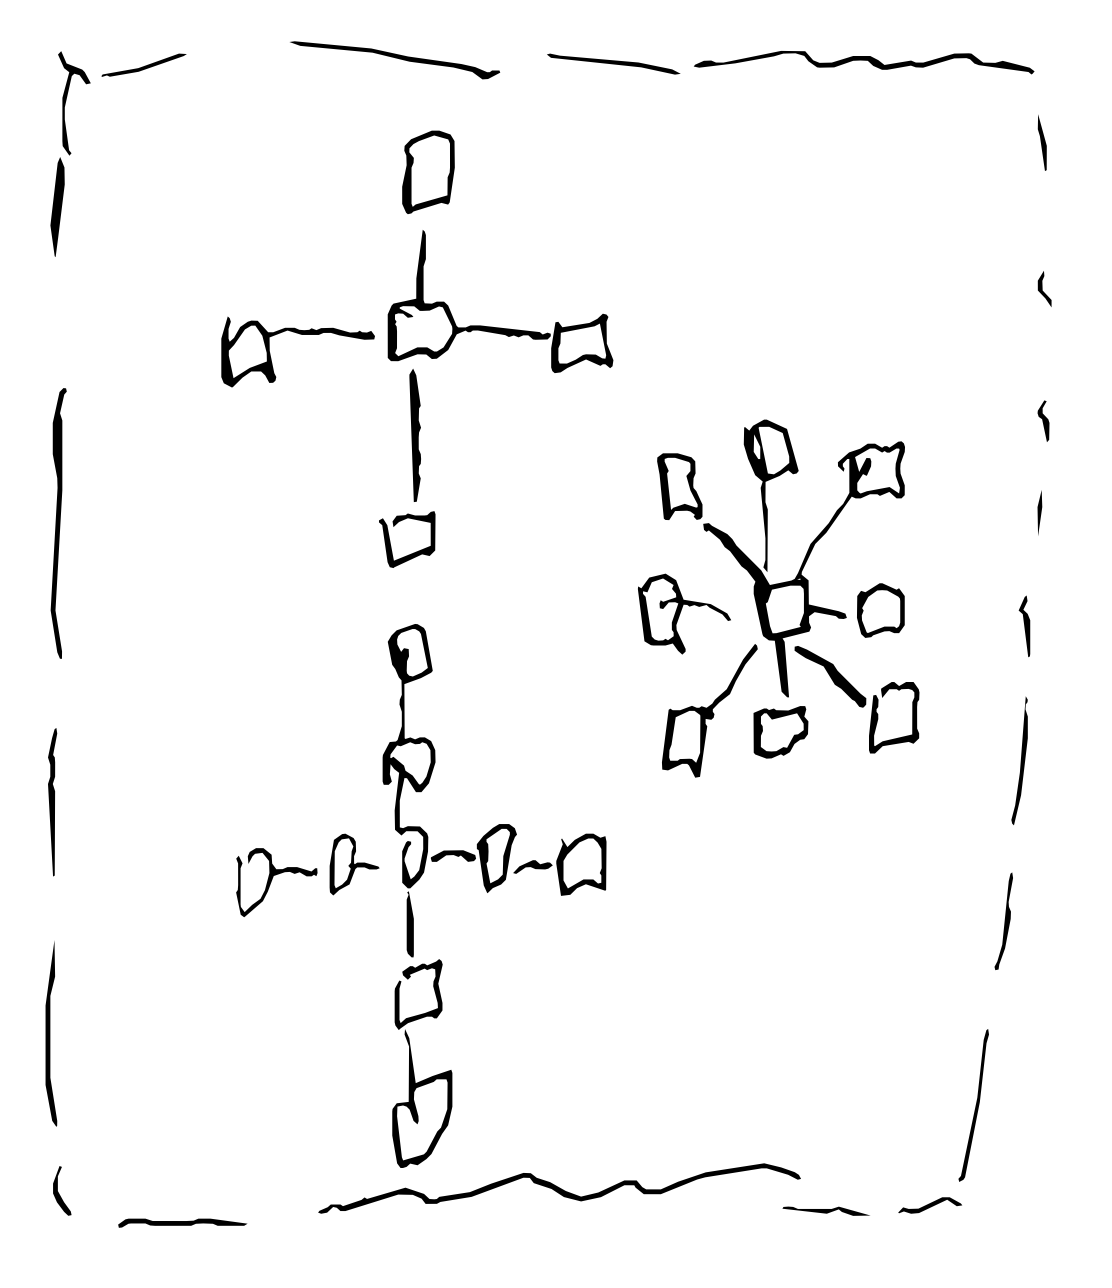
\includegraphics[width=4cm]{stencil_system_drawn.png}
\end{columns}
\end{frame}

\subsection{Domain}
\begin{frame}{Domain}
\begin{columns}
\column{0.48\linewidth}
\centering
\begin{outline}
  \1 Node graph / connectivity
  \1 May be geometry driven
  \1 Should be programmable (?)
    \2 Condensation problems 
  \1 Lots of axis aligned boxes in practice
  \1 Might include ``coloring'' to map different stencils
  \1 Where do want to sample?
  \1 Durating of runtime 
    \2 How often do we sample?
\end{outline}
\column{0.48\linewidth}
\centering
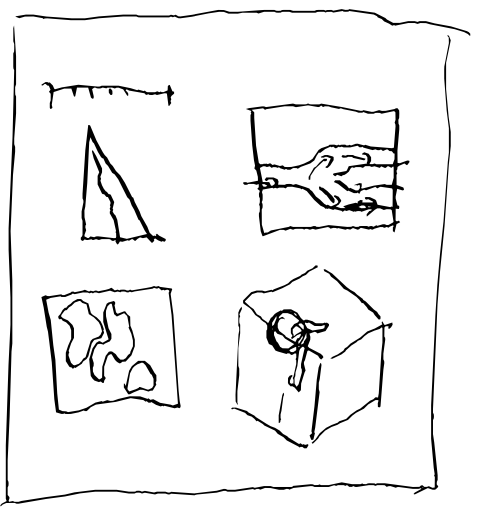
\includegraphics[width=4cm]{domain_drawn.png}
\end{columns}
\end{frame}

\subsection{Boundary Conditions}
\begin{frame}{Boundary Conditions}
\begin{columns}
\column{0.48\linewidth}
\centering
\begin{outline}
  \1 Fully programmable
    \2 Highly dependent on domain and stencil system
  \1 May require sampling
    \2 Outflow boundary conditions
    \2 Coupling to other simulations
\end{outline}
\column{0.48\linewidth}
\centering
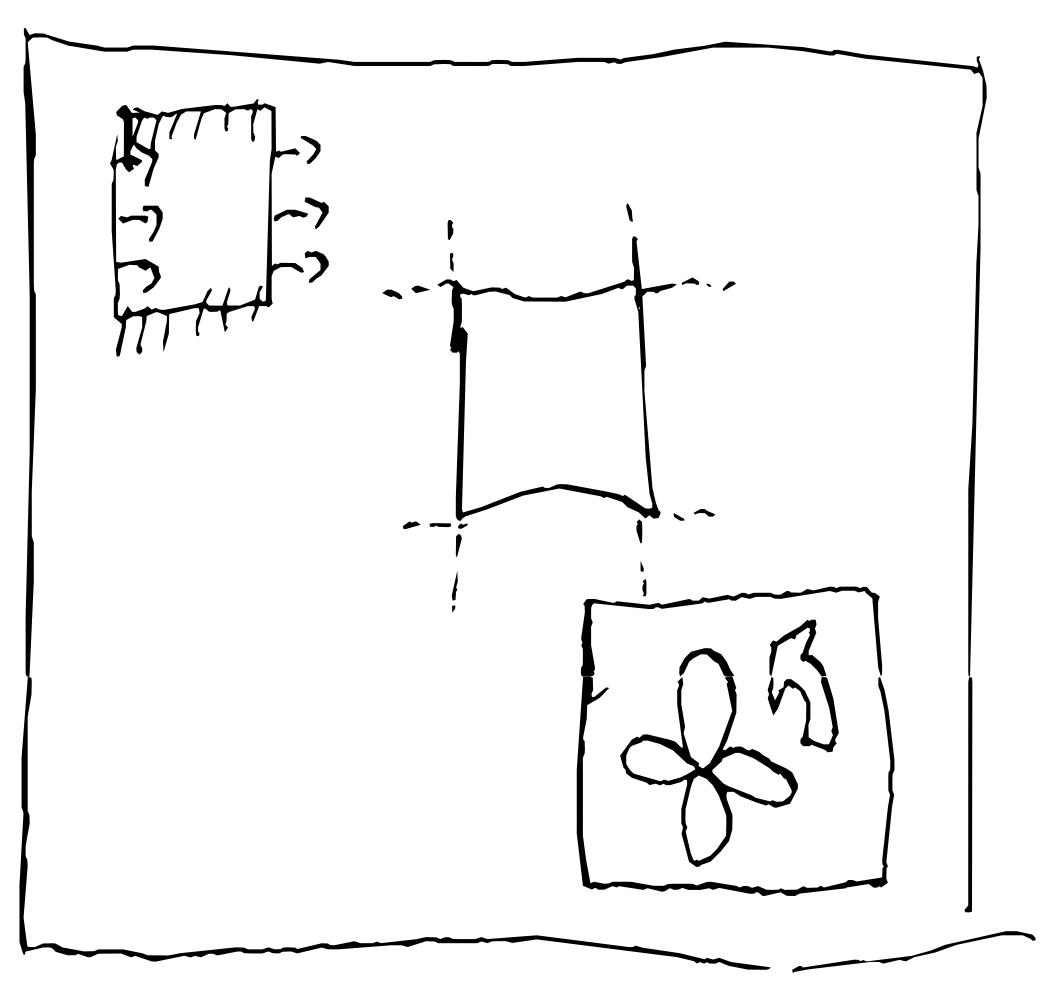
\includegraphics[width=4cm]{bc_drawn.png}
\end{columns}
\end{frame}

\section{Compilation Techniques}
\subsection{FFT}
\begin{frame}{FFT}
\begin{outline}
  \1 FFT algorithms \cite{Ahmad2021} \cite{Ahmad2023} \cite{Ahmad2023}
\end{outline}
\end{frame}

\subsection{Guassian Approximation}
\begin{frame}{Guassian Approximation}
\begin{outline}
  \1 Guassian Approximation \cite{Ahmad2022Brief}
\end{outline}
\end{frame}

\subsection{Polyhedral Compiling}
\begin{frame}{Polyhedral Compilers}
\begin{columns}
\column{0.48\linewidth}
\centering
\begin{outline}
  \1 PLUTO \cite{Bondhugula2008}, \cite{Bondhugula2008Pract}
    \2 C source to source compiler
    \2 Access optimized with tiling
  \1 LLVM Polygeist \cite{Moses2021} 
    \2 C++ / C interface to MLIR \cite{Lattner2021}
    \2 MLIR polyhedral optimization passes
  \1 LLVM Polly \cite{Grosser2012} 
    \2 Polyhedral optimization of LLVM IR
\end{outline}
\column{0.48\linewidth}
\centering
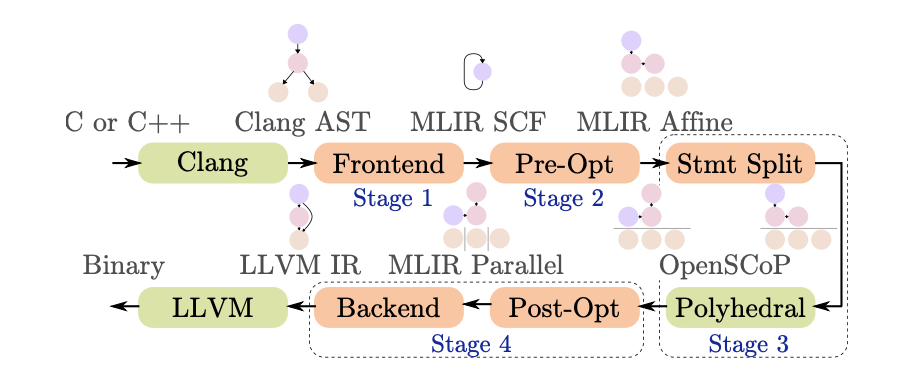
\includegraphics[width=4cm]{../../assets/polygeist_workflow.png}

Polygeist workflow

\end{columns}
\end{frame}

\subsection{Misc Techniques}
\begin{frame}{Misc Techniques}
\begin{outline}
  \1 Branch Removal
    \2 If statements may have arithmetic based alternative
  \1 Vectorizing
  \1 Data layout / Access patterns (AoS <-> SoA)
\end{outline}
\end{frame}

\section{Autotuner}
\begin{frame}
\begin{outline}
  \1 Profiling?
  \1 Plan Composition
  \1 Algorithm Tradeoffs
  \1 Other hyper parameters?
\end{outline}
\end{frame}

\section{Related}

\begin{frame}{Related Projects}
\begin{outline}

  \1 FFTW  \cite{Frigo2005}
    \2 Fast fourier transform compiler
    \2 A dependency(?) for SALTAR
    \2 Similiar architectural concerns
  \1 Taichi \cite{Hu2019}
    \2 JIT compiler parallel numerical code
    \2 Optimizes computation over sparse data
    \2 DSL is based on python.
  \1 Eigen \cite{eigenweb}
    \2 Runtime vs compile time configuration
  \1 FEnics \cite{Barrata2023} 
    \2 Compiler framework for FEA
\end{outline}
\end{frame}

\begin{frame}{Related Algorithms}
\begin{columns}
\column{0.58\linewidth}
\centering
\begin{outline}
  \1 HashLife \cite{Gosper1984}
    \2 Memoized Algorithm for cellular automata
    \2 Sensitive to entropy
  \1 Quicklife (Open Source with Golly)
    \2 Tree based evaluation
    \2 No hashing
\end{outline}
\column{0.38\linewidth}
\centering
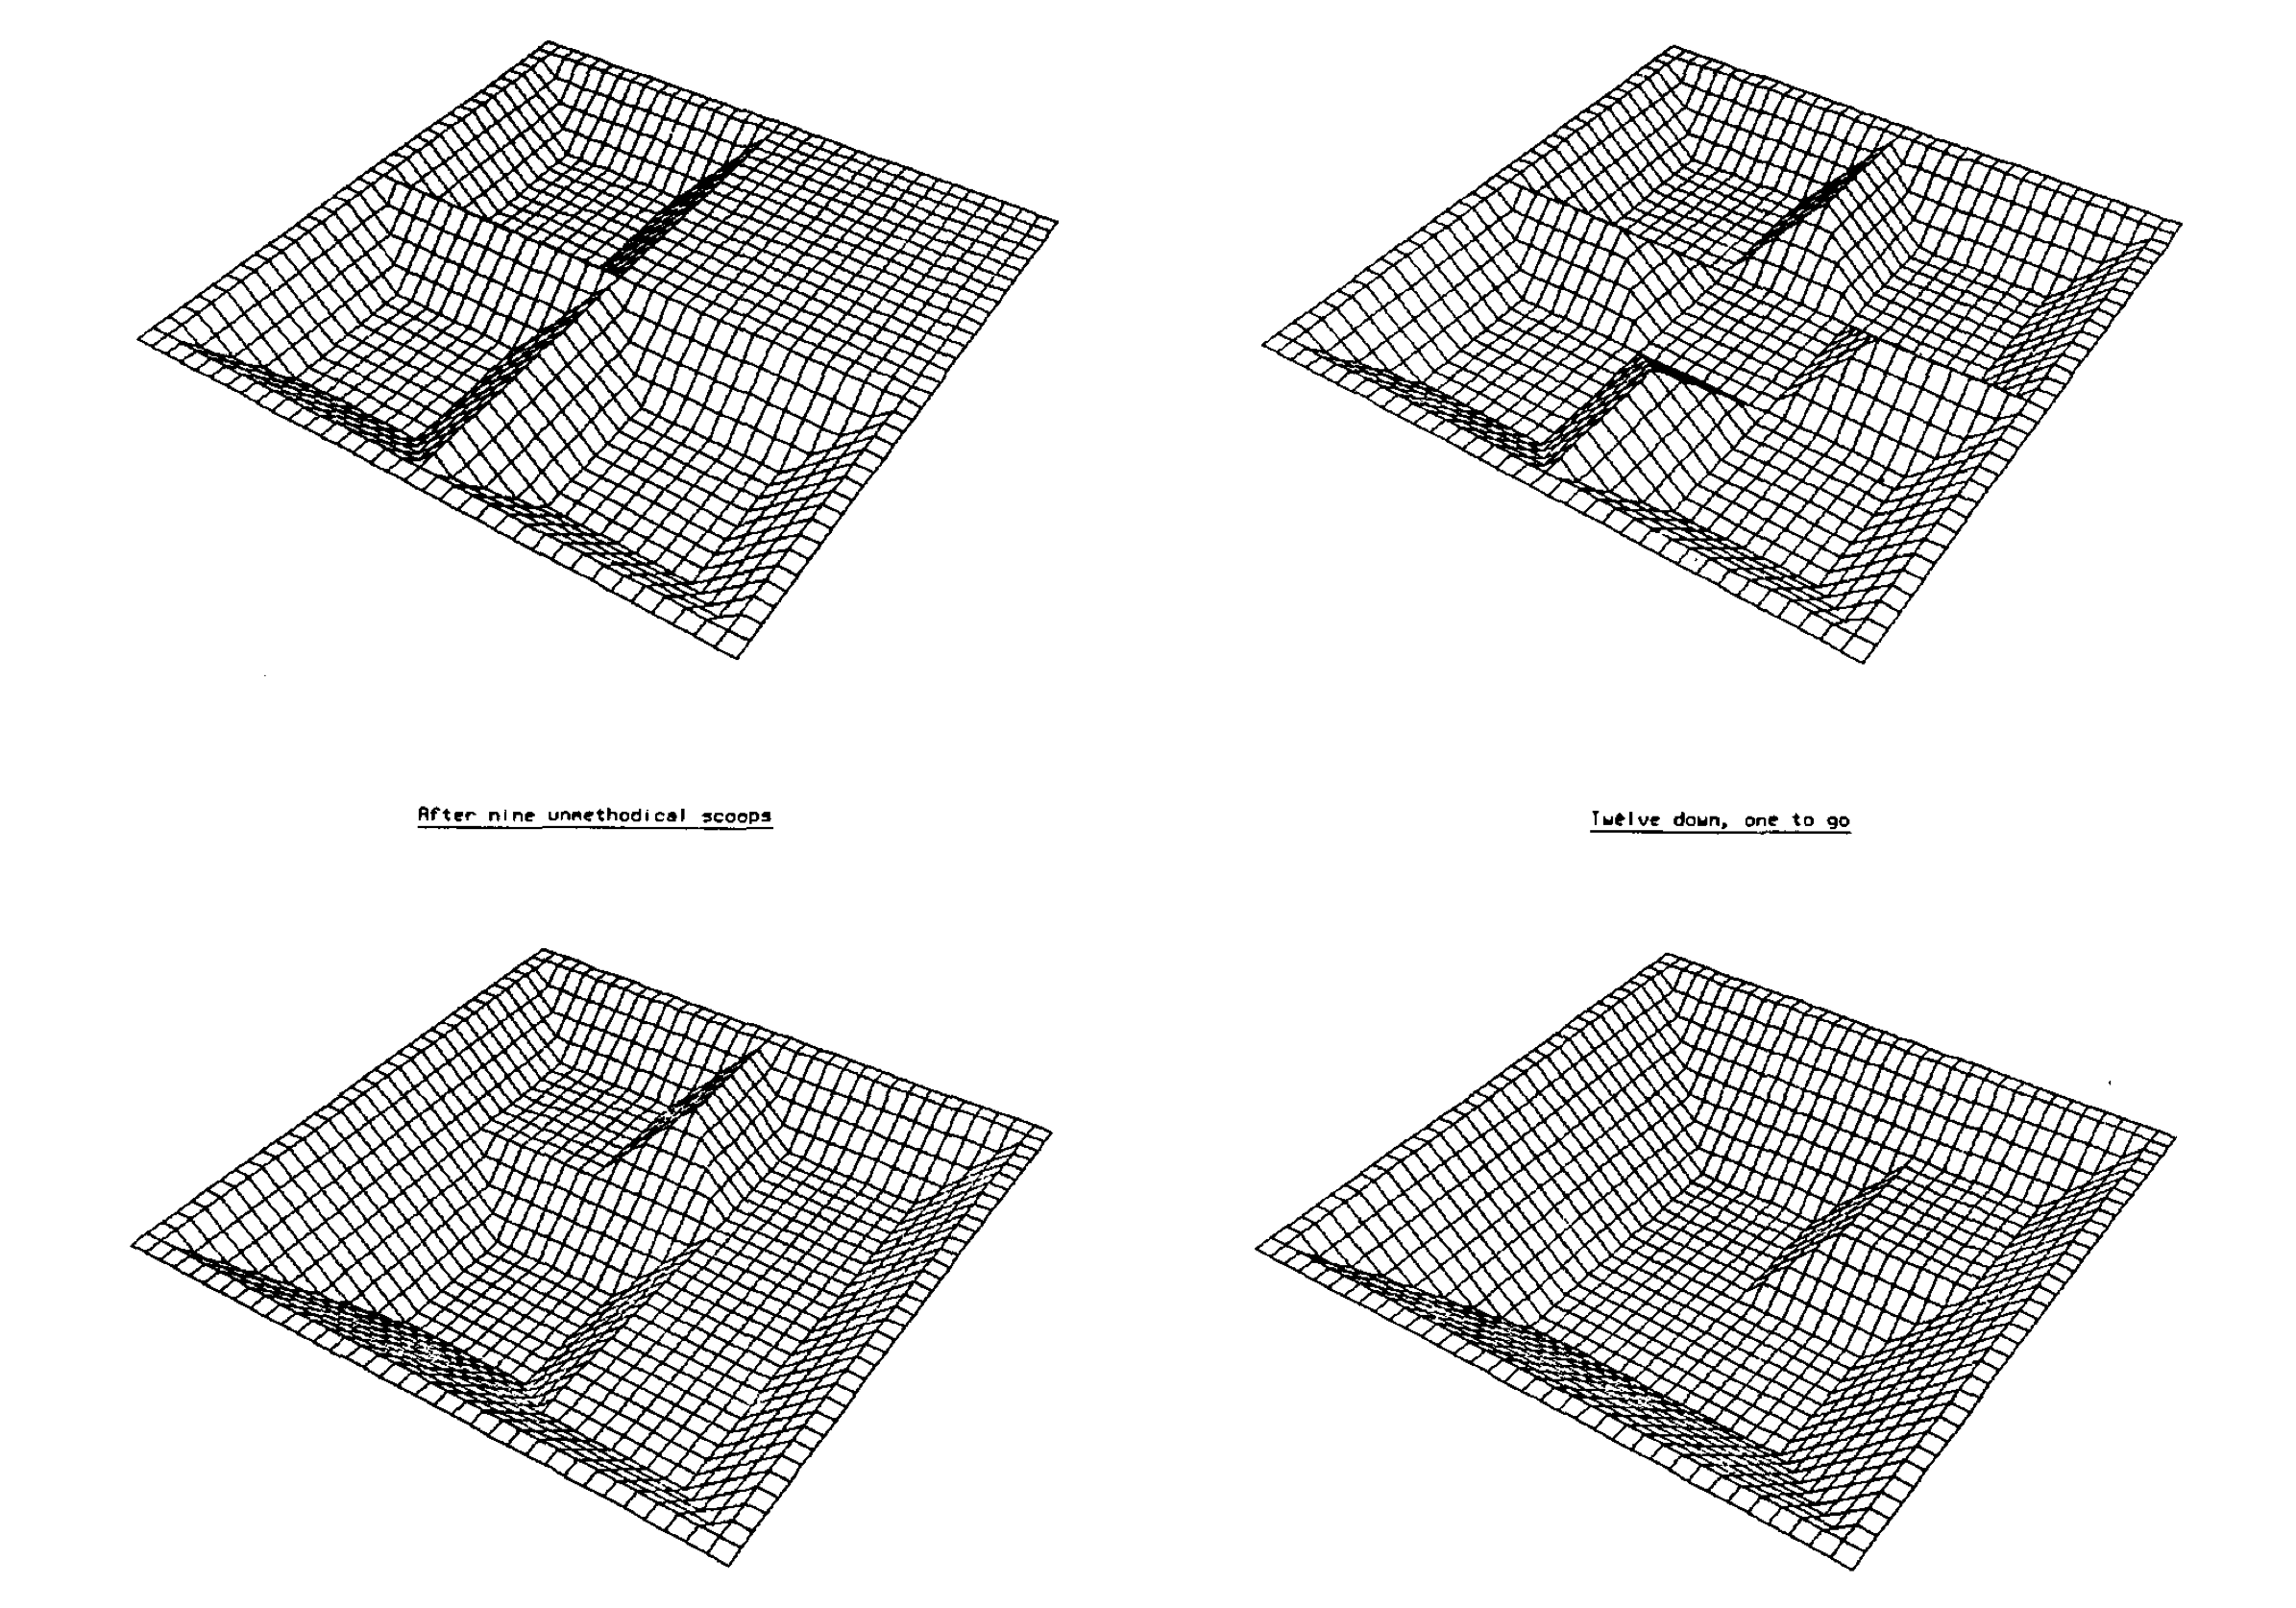
\includegraphics[width=4cm]{../../assets/hashlife_figure.png}
\end{columns}
\end{frame}


\begin{frame}[allowframebreaks]{References}
    \tiny
    \printbibliography
\end{frame}

\end{document}

